\chapter{Introduction}

\par In this thesis, I discuss the physics of matter in close proximity to neutron stars and black holes.  These astrophysical entities, collectively referred to as `compact objects',  are amongst the most extreme objects in our universe, consisting of several solar masses of matter compressed into an area $\lesssim20$\,km across.  These extreme densities are of interest to material physicists, as understanding matter in this regime requires entirely new equations of state.  The environments around these systems have extreme gravitational fields, meaning that these objects are also natural laboratories to test the limits of the theory of general relativity \citep{Einstein_GR}.  Additionally, neutron stars are strongly magnetic, piquing the interest of those interested in the dynamics of matter in extreme electromagnetic fields.  As the study of such objects is of interest to so many physical disciplines, understanding these objects is important to test the limits of our understanding of physics as a whole.
\par Unfortunately, compact objects are inherently faint objects; indeed, an isolated black hole is theoretically only visible via the effects its gravitational well has on the light from more distant stars.  As such, observational research into these objects tends to focus one of two types of system: Active Galactic Nuclei (AGNs) and X-Ray Binaries (XRBs).  In both of these types of system a compact object gravitationally attracts matter from its enviroment, a process known as `accretion'.  The act of matter falling into such a steep gravitational well causes large amounts of energy to be released; as such, these systems shine brightly in high-energy parts of the electromagnetic spectrum such as the X-rays and $\gamma$-rays.
\par AGNs contain supermassive black holes, with masses upwards of $\sim10^6$\,$M_\odot$\footnote{1\,$M_\odot\approx2\times10^{30}$\,kg, or one times the mass of our Sun.}.  These black holes are present at the centre of almost all large galaxies but many, such as Sagittarius A$^\star$ in our Milky Way, are currently dormant and not significantly accreting.  AGN are the brightest persistent sources of electromagnetic radiation in the universe, and they launch powerful `jets' of matter out to distances of many kiloparsec (kpc\footnote{$1$\,kpc$ =1000$\,parsec $\approx3\times10^{16}$\,m.  A parsec is the distance of an object that shows a parallax of 1'' (1 arcsecond, or $\frac{1}{3600}$ of a degree) against background objects when viewed from opposing points along the orbit of the Earth.}).  AGN have been implicated as having an important role in the development of their host galaxies via a process known as AGN feedback, in which mechanical and electromagnetic power from the AGN is `fed back' into its host galaxy and influences its evolution.
\par Active Galactic Nuclei are, almost by definition, very distant systems.  Because of the large size of these objects, they also only evolve over timescales of thousands of years.  These facts make studying the properties of matter in a relativistic regime by observing AGN somewhat difficult.  Thankfully, there exists a population of bright, accreting compact objects much closer to home: XRBs.

\section{Anatomy of an X-Ray Binary}

\par In this thesis, I will be focusing on XRBs.  These systems are physically much smaller than AGN, with compact objects no more massive than $\sim20\,M_\odot$, but in many ways they can be more extreme.  The gravitational tidal forces close to the compact object are greater than in AGN and, due to their small size, XRBs can evolve rapidly over timescales of seconds or less.

\subsection{Types of X-Ray Binaries: High and Low-Mass}

\par An XRB is a system containing a compact object\footnote{A black hole or a neutron star.  Similar systems with a white dwarf as their compact object are referred to as Cataclysmic Variables (CVs).} and a main sequence or giant companion star.  By various processes, matter is lost from the companion star and transferred onto the compact object.  Due to angular momentum constraints matter cannot simply fall onto the compact object; instead this matter spirals inwards, forming a large disk of material.  Frictional forces in the inner portions this disk heat this disk to extreme temperatures $\gtrsim1$\,keV\footnote{1\,keV$=1000\,eV=1.6\times10^{-19}$\,J .  1\,eV (electron-Volt) is the amount of energy an electron gains by crossing a potential difference of 1\,V.  Although this is a unit of energy, it is often used in high-energy physics to denote temperature by describing the energy at which the emission of a black body at that temperature is peaked.  1\,keV corresponds to a temperature of $\sim1.16\times10^7$\,K}.  In some XRBs, so much X-ray radiation is released in this process that the pressure from photons, which is negligible but non-zero under standard conditions, becomes important to describe the equation of state of the disk.
\par XRBs are divided into two broad categories depending on the mass of the companion star and, in turn, the predominant mechanism responsible from transferring matter from the star to the compact object.  High Mass X-ray Binaries (HMXBs) have a companion star with a mass $\gtrsim1\,M_\odot$.  High mass stars tend to be unstable, and these objects can eject large quantities of matter in a stellar wind.  In a HMXB, part of this stellar wind is gravitationally captured by the compact object and feeds the accretion disk.
\par Low Mass X-Ray Binaries, systems in which the mass of the companion star is $\lesssim1\,M_\odot$, accrete matter in a different way.  Objects in astrophysical binary systems each have a Roche Lobe: a teardrop-shaped region of space in which that object is gravitationally dominant.  Inside the Roche Lobe matter is gravitationally bound to the star, while matter outside of the lobe is free to escape to infinity or to accrete onto another nearby object.
\par Under some circumstances, it is possible for a star to become larger than its Roche lobe.  This can happen in two main ways:
\begin{enumerate}
\item The size of the binary orbit decreases, shrinking the Roche Lobe of each object.
\item The radius of the star increases.  This can happen, for example, when the star evolves from the Main Sequence onto the Giant branch.
\end{enumerate}
In either scenario, a portion of the star ends up within the Roche lobe of the compact object.  This matter is free to spiral onto the compact object, forming the accretion disk.

\subsection{Components of an X-Ray Binary}

\par As well as the accretion disk, there are several additional features present in a typical X-Ray Binary; we show a cartoon diagram of an LMXB in Figure \ref{fig:xrbcartoon}.   Radio observations of nearby XRBs have shown that these systems can show axial jets of material similar to those seen in AGN \citep{Geldzahler_Jet}; in Figure \ref{fig:jet} we show a radio image from \citet{Stirling_Jet} showing a jet from the HMXB Cyg X-1. These jets can eject matter at velocities approaching the speed of light (e.g. \citealp{Mirabel_Microquasar}).

\begin{figure}
    \includegraphics[width=\columnwidth, trim = 0mm 0mm 0mm 0mm]{images/xrbcartoon.eps}
    \captionsetup{singlelinecheck=off}
    \caption[A cartoon illustrating the basic geometry of a simple X-ray binary.]{A cartoon illustrating the basic geometry of a simple X-ray binary.  Not shown is the non-thermal corona of material which can be inferred from spectroscopy, as the geometry of this feature is disputed.  Diagram not to scale.}
   \label{fig:xrbcartoon}
\end{figure}

\begin{figure}
   \centering
    \includegraphics[width=0.5\columnwidth, trim = 17mm 0mm 17mm 0mm, clip]{images/jet.eps}
    \captionsetup{singlelinecheck=off}
    \caption[An 8\,GHz radio image from \citet{Stirling_Jet} showing a jet from the HMXB Cyg X-1.]{An 8\,GHz radio image from \citet{Stirling_Jet} showing a jet from the HMXB Cyg X-1 (at the origin of the image).  The lowest countour is 0.4\,mJy\,beam$^{-1}$, and other contours represent factors of 2.}
   \label{fig:jet}
\end{figure}

\par X-ray spectral studies of LMXBs find that, in addition to a black-body\footnote{The energy spectrum of a black body at temperature $T$ is given by \[F_T(\nu)=\frac{N\nu^3}{e^\frac{h\nu}{k_BT}-1}\] for some constant $N$ \citep{Planck}.  $k_B$ is the Boltzmann Constant, and $c$ is the speed of light in a vacuum.} like accretion disk, the systems must each contain a non-thermal `corona' component.  This corona emits X-rays via Compton upscattering.  In this process, photons emitted from the disk collide with energetic electrons in the corona.  The photons, on average, gain energy from these collisions and are scattered back into space; some in the direction of observers on the Earth.  This leads to a characteristic power-law\footnote{A power-law distribution is any distribution with the functional form $f(x)=cx^k$ for some constants $c$ and $k$.} energy distribution signature at high energies, which can be seen in the spectra of LMXBs.  As we show in the simulated LMXB energy spectrum in Figure \ref{fig:toyspec}, the emission from the corona tends to dominate above energies of $\sim10$\,keV.
\par Models of the geometry of the coronal region have evolved over the years.  While the corona has been historically treated as if it was a single point fixed above the centre of the disk (the so-called `Lamp Post' model, e.g. \citealp{Rozanska_Lamppost}), more recent models tend to treat it either as an optically thin\footnote{An optically thin medium is defined as a medium in which an average photon interacts $<1$ times while passing through.} flow of material onto the compact object or equate it with the base of the radio jet (e.g. \citealp{Skipper_CoronaGeo}).

\begin{figure}
   \centering
    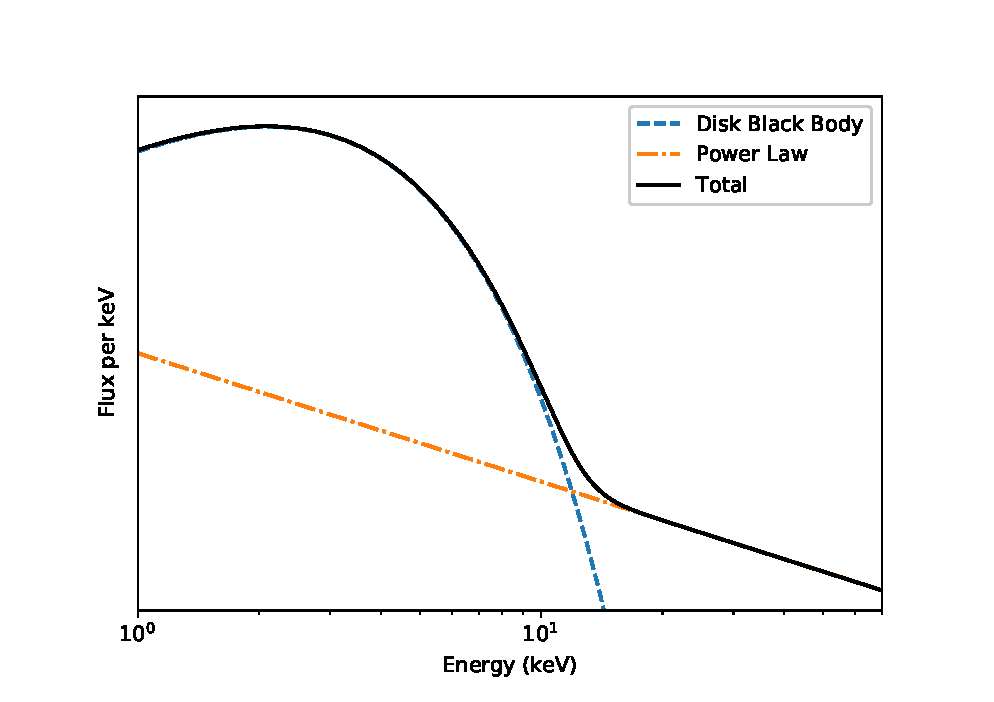
\includegraphics[width=0.7\columnwidth, trim = 10mm 0mm 10mm 10mm, clip]{images/toy_spec.eps}
    \captionsetup{singlelinecheck=off}
    \caption[A simulated, simplified spectrum of an LMXB, showing the two main components visible in X-ray: the accretion disk and the corona.]{A simulated, simplified spectrum of an LMXB, showing the two main components visible in X-ray: the accretion disk (blue) and the corona (orange).  The disk is generally modelled as a disk black body, a sum of black bodies at different temperatures corresponding to different annuli in the disk (e.g. \citealp{Mitsuda_diskbb}), while the corona is modeled as a power law.}
   \label{fig:toyspec}
\end{figure}

\par Another important component of an X-ray binary is the disk wind.  Due to the high temperatures and pressures in the inner part of the accretion disk, matter on the surface of the disk can obtain enough energy to escape the gravitational well of the compact object.  This matter is ejected from the system in large-scale, high velocity winds; studies of the spectral lines present in these winds have shown that they can have speeds approaching the speed of light (e.g. \citealp{Degenaar_BPSpec}).

\subsubsection{Neutron Star X-ray Binaries}

\label{sec:NSintro}

\par The geometry of an X-ray binary is somewhat more complicated when the compact object is a neutron star.  Unlike black holes, neutron stars are in general highly-magnetised systems, and the introduction of a large, strong magnetic field to an XRB has implications for the geometry of the accretion flow.  At some point in the inner accretion disk, it is possible that the pressure exerted by this magnetic field becomes dominant over the gas and photon pressures.  At this point, ionised material becomes `frozen-in' to the magnetic field lines, and is only able to freely move along them; due to the extreme temperatures in the inner portion of the accretion disk, the vast majority of material in this region is ionised.  The result of this effect is a disruption of the flow in the inner part of the accretion disk, in which matter is funneled along field lines and onto the poles of the neutron star.  This causes the poles of the neutron star to become extremely hot; as the neutron star spins, it appears to pulse as seen by an external observer due to the magnetic poles coming in and out of view.  These objects are referred to as accreting X-ray pulsars.
\par In addition to the effects of the magnetic field, there is another significant difference between neutron star and black hole binaries.  Black holes are surrounded by an event horizon from which no light can emerge, meaning that the compact object in black hole X-ray binaries cannot be seen directly.  Neutron stars, on the other hand, have no such event horizon.  As such the surface of the neutron star itself, and any phenomena that take place there, can also be seen.
\par One of the most spectacular events that can occur on the surface of a neutron star is a Type I X-ray burst.  These occur when matter accreted onto the surface of the neutron star reaches a critical temperature and pressure, and nuclear fusion is triggered.  This results in a flash of energy, which causes a runaway thermonuclear explosion across all or most of the neutron star surface.  Type I bursts appear in data as a sudden $\sim1$--2 orders of magnitude increase in X-ray flux, followed by an power-law decay as the neutron star surface cools.  As Type I bursts are distinctive features which require a surface on which to occur, they are often used as a diagnostic tool to identify an unknown LMXB compact object as a neutron star.

\section{Low Mass X-Ray Binary Behaviour}

\par LMXBs are not static systems, and most show complex variability over timescales of milliseconds to years.  Broadly speaking, LMXBs can be divided into persistent systems and transient systems.  Persistent systems have always observed to be bright since their discovery, implying a constantly high rate of accretion.  In some objects, this bright, high-accretion rate state has persisted for at least $\geq20$ years (e.g. GRS 1915+105, \citealp{Deegan_1915}).
\par Transient LMXBs have a somewhat more complicated life cycle.  These objects spend most of their time in a ``quiescent'' state, during which they are faint in X-rays and only a small amount of material is being accreted.  However these objects also undergo ``outbursts'', during which they increase in intensity by many orders of magnitude for a period of days to months.  The frequency of these outbursts varies widely between sources, ranging from one every month or so to one every few decades or longer.
\par LMXB outbursts tend to follow a predictable path, evolving through a number of different `states' as they progress.  We show some of these states in Figure \ref{fig:Fender} on a so-called `hardness-intensity diagram', which traces how the brightness and the spectral shape of a source evolve over time (see Section \ref{sec:hids} for more information on hardness-intensity diagrams).  At the start of a typical outburst emission from the source is spectrally hard, i.e. dominated by higher-energy photons.  This part of the outburst is referred to as a Low/Hard State (bottom-right of Figure \ref{fig:Fender}), and a radio jet is generally visible at this time.  The luminosity of the source gradually increases until it reaches some maximum, and then emission begins to become softer as the system heads towards the High/Soft State (top-right of Figure \ref{fig:Fender}).  During this transition, the system crosses the so-called `jet line', and the radio jet switches off.  Sources tend to spend a large portion of their outbursts in the high/soft state, appearing to meander in the hardness-intensity diagram.  This meandering may include additional crossings of the jet line, causing the radio jet to flicker on and off during this period.  The X-ray luminosity of the source then decreases, before the source returns to the hard state along a path of approximately constant luminosity.  The source then fades back into quiescence.  This typical outburst behaviour forms a distinctive `q' shape in the hardness-intensity diagram, as we show in Figure \ref{fig:Fender}, and can be thought of as the inner accretion disk filling with matter before draining onto the compact object or out of the system in winds (e.g. \citealp{Fender_UniJets}).  This relatively complex evolution over the course of an outburst highlights the fact that accretion is not a simple process, and that understanding accretion gives us better understanding of a areas of the physics of matter in extreme environments.

\begin{figure}
   \centering
    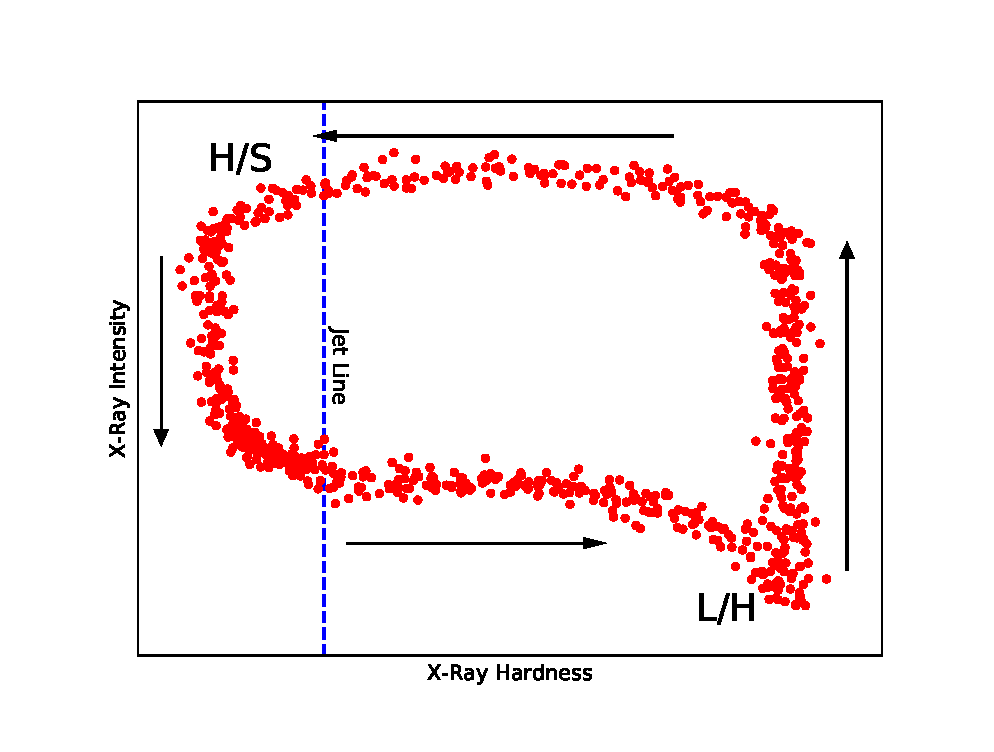
\includegraphics[width=\columnwidth, trim = 0mm 0mm 0mm 0mm, clip]{images/Fender_D.eps}
    \captionsetup{singlelinecheck=off}
    \caption[A cartoon hardness-intensity diagram adapted from \citet{Fender_UniJets}, showing the evolutionary path of a typical LMXB outburst.]{A cartoon hardness-intensity diagram adapted from \citet{Fender_UniJets}, showing the evolutionary path of a typical LMXB outburst and roughly indicating the positions of the Low/Hard (L/H) and High/Soft (H/S) States.  The jet line roughly demarcates the portion of the outburst in which a jet is observed (right of the line) from the portion in which it is not observed (left of the line).}
   \label{fig:Fender}
\end{figure}

\section{Relativistic Effects}

\par One of the most obvious extreme physical environments that accretion physics sheds light on is, of course, extreme gravitational fields.  General relativistic effects around compact objects are often expressed in relation to the gravitational radius $r_g$, defined as:

\begin{equation}
r_g=\frac{2GM}{c^2}
\end{equation}

Where $G$ is the gravitational constant, $c$ is the speed of light and $M$ is the mass of the compact object.  1$r_g$ is equal to the Schwarzchild radius, or the radius of the event horizon of a non-rotating black hole with mass $M$ \citep{Schwarzchild}.
\par One result of general relativity which is important when considering compact object accretion disks is the accretion of an Innermost Stable Circular Orbit, or ISCO.  This radius is at $3r_g$ from the centre of a non-rotating object, placing it well outside the event horizon of a black hole and above the surface of some neutron stars.  It can be shown that any isolated point mass crossing this boundary from the outside will continue into the black hole, whereas any point mass crossing it from the inside will continue to infinity; as such, no stable orbit can exist with a periastrion smaller than this radius. It can be shown that an accretion disk is also bounded by this radius \citep{Kozlowski_ISCO}, meaning that XRB accretion disks must all have an inner truncation radius at at least $3r_g$ from the compact object.
\par In general, a black hole can be described in 3 parameters\footnote{This conjecture is often referred to as the `No-Hair' theorem.}: in addition to mass, a black hole can possess non-zero angular momentum (or spin) and charge.  As the precursor stars to black holes are neutrally charged, it is expected that all astrophysical black holes are very close to being neutral as well.  However, these precursor stars also possess non-zero angular momentum.  As such, it is expected that most if not all astrophysical black holes are spinning.  This spin is generally expressed as a number between 0 and 1, where 0 denotes a non-rotating black hole and 1 is the maximum permitted angular momentum the object can possess.  General relativity tells us that this spin will also have a significant effect on accretion physics.  First of all, this spin serves to change the position of the ISCO; moving it to a maximum of $4.5r_g$ for a black hole with spin of 1.  A spinning black hole also distorts the space time around it, in a process known as frame-dragging.  This forces matter close to the black hole to orbit in the same plane as it.  As there is no reason to assume the outer disk orbits in the same plane as the black hole, this can lead to situations in which the accretion disk is warped, which in turn has implications for the flow of matter within it.
\par It is clear that the general relativity should have observable implications on the flow of matter onto the accretion disk.  Studying the physics of accretion therefore allows us to measure parameters such as the spin of black holes that would otherwise be inaccessible to us.  Additionally, a full understanding of the accretion onto the compact objects would allow us to look for discrepancies between what is observed and what is expected from relativity.  Therefore, a full understanding of accretion is one route to testing the theory of relativity itself under some of the most extreme conditions in the universe.